\documentclass[12pt, letterpaper]{article}
% must use this pkg for displaying imgs
\usepackage{graphicx}
\usepackage{amsmath}
\usepackage{multirow,array}
\usepackage{blindtext}
\usepackage{etoolbox}
\usepackage[a4paper, total={6in, 9in}]{geometry}
\graphicspath{ {../../imgs/} }
% pkg for links
\usepackage{hyperref}
% for codeblocks highlighting
\usepackage{listings}
\lstset{language=C}


\makeatletter
\patchcmd{\raggedright}{\parindent\z@}{}{}{}
\makeatother

\begin{document}


\newcommand{\paperauthor}{Akiel Aries}
\newcommand{\papersupervisor}{Prof. Sareh Assiri}
\newcommand{\paperuniversity}{Northern Arizona University}

\newcommand{\papertitle}{Analyzing Mirai}
\newcommand{\paperminortitle}{a Linux-Focused Attack}
\newcommand{\papermajorheading}{Cybersecurity}
\newcommand{\paperminorheading}{CYB 410 - Software Security}

\newcommand{\HRule}{\rule{\linewidth}{0.5mm}} % Defines a new command for the horizontal lines, change thickness here

\center % Center everything on the page

%----------------------------------------------------------------------------------------
%	HEADING SECTIONS
%----------------------------------------------------------------------------------------

\textsc{\LARGE \paperuniversity}\\[1.0cm] % Name of your university/college
\textsc{\Large \papermajorheading}\\[0.2cm] % Major heading such as course name
\textsc{\large \paperminorheading}\\[0.75cm] % Minor heading such as course title

%----------------------------------------------------------------------------------------
%	TITLE SECTION
%----------------------------------------------------------------------------------------

\HRule \\[0.4cm]
{ \huge \bfseries \papertitle}\\[0.05cm] % Title of your document
{ \huge \paperminortitle}\\[0.025cm] % Title of your document
\HRule \\[3.5cm]

\begin{center}
	\makebox[1.0\textwidth]{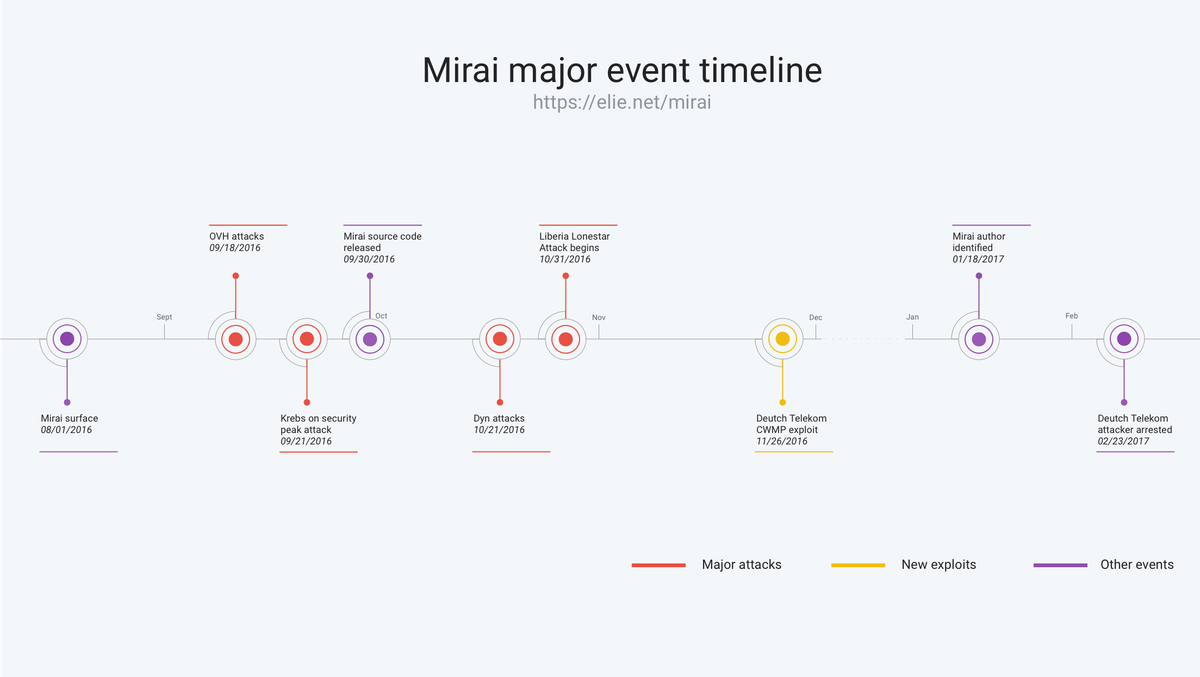
\includegraphics[width=1.0\textwidth]{mirai-major-events-timeline.png}}
\end{center}


\vfill % Fill the rest of the page with whitespace
%----------------------------------------------------------------------------------------
%	AUTHOR SECTION
%--------------------------------------------------------------------------------------

\begin{minipage}{0.4\textwidth}
	\begin{flushleft} \large
	\emph{Author:}\\
	\paperauthor
	\end{flushleft}
	\end{minipage}
	~
	\begin{minipage}{0.4\textwidth}
	\begin{flushright} \large
	\emph{Professor:} \\
	\papersupervisor
	\end{flushright}
\end{minipage}\\[1cm]

%----------------------------------------------------------------------------------------
%	DATE SECTION
%----------------------------------------------------------------------------------------
{\large \today}\\ % Date, change the \today to a set date if you want to be precise

\newpage

\begin{sloppypar}


% classification img
%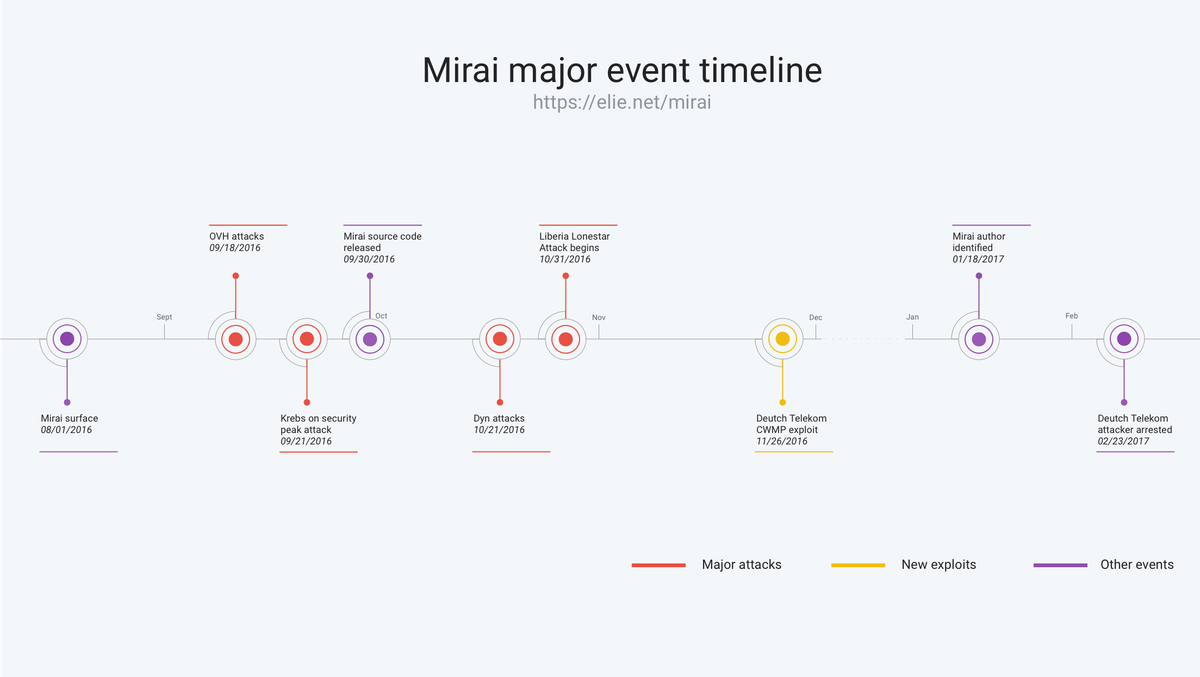
\includegraphics[scale=0.3]{mirai-major-events-timeline.png}
\begin{flushleft}
\section{Overview}
Mirai is a piece of malware targeting IoT (Internet of Things) devices first discovered 
in 2016 by a malware research group MalwareMustDie and gaining more popularity when 
cybersecurity journalist Brian Krebs' website was attacked. The goal being to 
control nodes part of a botnet running large-scale attacks. From previous research on 
attack history most victims include consumer grade devices such as local home routers 
and IP cameras, which are known to be insecure and attack-prone. The bot has been used 
in very large-scale DDoS (Distrubuted Denial of Service) atacks targeting many users 
machines and taking place accross the globe. Mirai's networking agent is written in C 
and its controller interface written in Go. It utilizes computer numerical control (CNC) 
which is a quite genius way to control the operation and functionality of a machine 
through injection of software. Since being discover and its source code leaked, Mirai 
went on to spawn many variations, much like pieces of malware, that exploited zero-day's 
in some pieces of software for effecient and malicious operation. In recent news, on
October 14th 2022, it was reported that the Wynncraft Minecraft server was hit with
a 2.5 Tbps DDoS attack lasting about 2 minutes in total. As we go in depth we will see
why this number is absurd. 

%\newpage

\section{Source Code}
The scanner.c file does most of the initializing and calling of source. So within this
file the first thing that caught my attention was the \verb|void scanner_init(void)| 
function. In the function we can see a series of \verb|add_auth_entry| calls that add 
in usernames as well as password to perform a dictionary attack to sign in to insecure
IoT devices. Which seems to be the biggest fix to preventing this piece of malware from
infecting your system, using a somewhat secure password!

\begin{lstlisting}
// Set up passwords
// root     xc3511
add_auth_entry("\x50\x4D\x4D\x56", 
"\x5A\x41\x11\x17\x13\x13", 10);
// root     vizxv
add_auth_entry("\x50\x4D\x4D\x56", 
"\x54\x4B\x58\x5A\x54", 9);
// root     admin
add_auth_entry("\x50\x4D\x4D\x56",
"\x43\x46\x4F\x4B\x4C", 8);
// admin    admin
add_auth_entry("\x43\x46\x4F\x4B\x4C", 
"\x43\x46\x4F\x4B\x4C", 7);
// root     888888
add_auth_entry("\x50\x4D\x4D\x56", 
"\x1A\x1A\x1A\x1A\x1A\x1A", 6);
// root     xmhdipc
add_auth_entry("\x50\x4D\x4D\x56", 
"\x5A\x4F\x4A\x46\x4B\x52\x41", 5);
// root     default
add_auth_entry("\x50\x4D\x4D\x56", 
"\x46\x47\x44\x43\x57\x4E\x56", 5);
\end{lstlisting}

Interesting enough, within the scanner.c file some addresses are hardcoded not to visit 
when performing the IP scan for inital infection. The Department of Defense, the US Postal
Service, GE, HP as well as the Internet Assigned Numbers Authority (IANA) + more were 
deemed as invalid for scanning.

\begin{lstlisting}
static ipv4_t get_random_ip(void) {
    uint32_t tmp;
    uint8_t o1, o2, o3, o4;

    do {
        tmp = rand_next();

        o1 = tmp & 0xff;
        o2 = (tmp >> 8) & 0xff;
        o3 = (tmp >> 16) & 0xff;
        o4 = (tmp >> 24) & 0xff;
    }
    while (o1 == 127 || // 127.0.0.0/8      - Loopback
          // 0.0.0.0/8		- Invalid address space
          (o1 == 0) || 
          // 3.0.0.0/8		- General Electric Company
          (o1 == 3) || 
          // 15.0.0.0/7		- Hewlett-Packard Company
          (o1 == 15 || o1 == 16) || 
          // 56.0.0.0/8       - US Postal Service
          (o1 == 56) || 
          // 10.0.0.0/8       - Internal network
          (o1 == 10) || 
          // 192.168.0.0/16   - Internal network
          (o1 == 192 && o2 == 168) ||
          // 172.16.0.0/14    - Internal network
          (o1 == 172 && o2 >= 16 && o2 < 32) ||
          // 100.64.0.0/10    - IANA NAT reserved
          (o1 == 100 && o2 >= 64 && o2 < 127) ||
          // 169.254.0.0/16   - IANA NAT reserved
          (o1 == 169 && o2 > 254) ||
          // 198.18.0.0/15    - IANA Special use
          (o1 == 198 && o2 >= 18 && o2 < 20) ||
          // 224.*.*.*+       - Multicast
          (o1 >= 224) ||
		  /*
		   * 6.0.0.0/7		- Department of Defense 
		   * 11.0.0.0/8 	- Department of Defense
		   * 21.0.0.0/8 	- Department of Defense
		   * 22.0.0.0/8 	- Department of Defense
		   * 26.0.0.0/8 	- Department of Defense
		   * 28.0.0.0/7 	- Department of Defense
		   * 30.0.0.0/8 	- Department of Defense
		   * 33.0.0.0/8 	- Department of Defense
		   * 55.0.0.0/8 	- Department of Defense
		   * 214.0.0.0/7	- Department of Defense
		  /*          
          (o1 == 6 || o1 == 7 || o1 == 11 || o1 == 21 
          || o1 == 22 || o1 == 26 || o1 == 28 
          || o1 == 29 || o1 == 30 || o1 == 33 
          || o1 == 55 || o1 == 214 || o1 == 215) 
          
    );

    return INET_ADDR(o1,o2,o3,o4);
}

\end{lstlisting}
Mirai uses many techniques to hide it's identity and what I found the most
naive method to be was the spoofing of user agents specifically these:
\begin{verbatim}
Mozilla/5.0 (Windows NT 10.0; WOW64) 
AppleWebKit/537.36 (KHTML, like Gecko) 
Chrome/51.0.2704.103 Safari/537.36

Mozilla/5.0 (Windows NT 10.0; WOW64) 
AppleWebKit/537.36 (KHTML, like Gecko) 
Chrome/52.0.2743.116 Safari/537.36

Mozilla/5.0 (Windows NT 6.1; WOW64) 
AppleWebKit/537.36 (KHTML, like Gecko) 
Chrome/51.0.2704.103 Safari/537.36

Mozilla/5.0 (Windows NT 6.1; WOW64) 
AppleWebKit/537.36 (KHTML, like Gecko) 
Chrome/52.0.2743.116 Safari/537.36

Mozilla/5.0 (Macintosh; Intel Mac OS X 10_11_6) 
AppleWebKit/601.7.7 (KHTML, like Gecko) 
Version/9.1.2 Safari/601.7.7
\end{verbatim}


Since Mirai is a DDOS bot, there are many spots in the code base of the bug that 
references some networking principles. The OSI (Open Systems Interconnection) model 
depicting the functions of a networking system. For now, let's take a look at how
Mirai makes use of layer 3, network. 
\begin{center}
{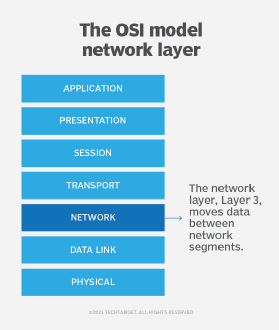
\includegraphics[width=0.5\textwidth]{osi-networking.png}}
\end{center}

Mirai makes use of launching GRE IP (Generic Routing Encapsulation) \& GRE ETH floods
in conjunction with SYN \& ACK floods. Another important piece of the code is the 
hardcoding/bypassing taking place that implies more security risks. The GRE floods
when analyzed closely peak at approximately 280 Gbps.

\begin{center}
{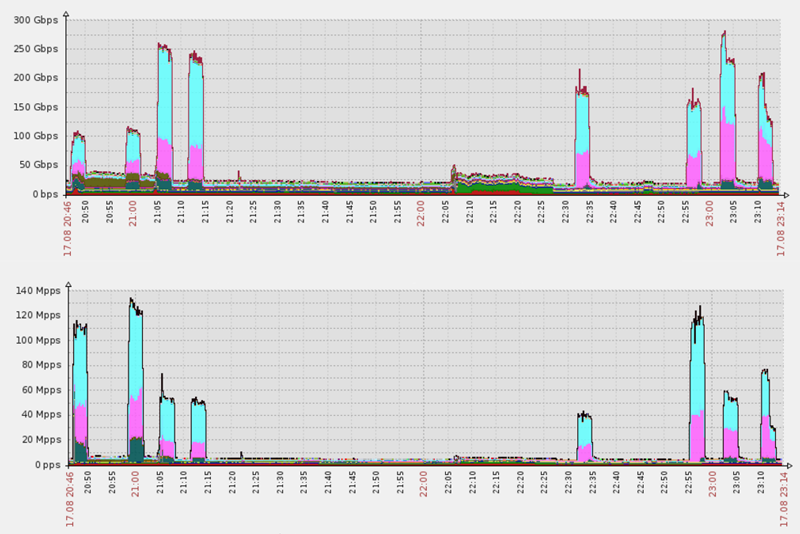
\includegraphics[width=0.8\textwidth]{mirai-bandwidth.png}}
\end{center}

This loop iterates through the ACK + SEQ numbers that are retrieved. SEQ is the value
sent by a TCP client that specifies the amount of data sent in the session. ACK is the 
value returned by the TCP server that indicates data has been recieved and is ready to
begin the next segment. 

\begin{lstlisting}
// Retrieve all ACK/SEQ numbers
for (i = 0; i < targs_len; i++) {
    int fd;
    struct sockaddr_in addr, recv_addr;
    socklen_t recv_addr_len;
    char pktbuf[256];
    time_t start_recv;

    stomp_setup_nums:
\end{lstlisting}

This particular piece of the tcp attack file caught my attention and I found
that 0xffffffff is a Windows update error returning when the update fails to search 
or install. 

\begin{lstlisting}
if (source_ip == 0xffffffff)
	iph->saddr = rand_next();
\end{lstlisting}

%\newpage

\section*{Scale}
On just the first day, it was said that upwards of 60,000 IoT devices were infected and at
its peak infected more than 600,000 devices. As previously stated many of these targets
were IP cameras. It was reported that the Mirai virus was located in 160+ countries. Of the
devices that were infected, routers and cameras made up the majority. \\

Overview of infiltration:
\begin{center}
\begin{table}[ht]
  \large  
  \centering 
  \renewcommand{\arraystretch}{1.5}
  \begin{tabular}{c|c||*{8}{c|}}
\cline{2-6}
&& \bfseries HTTPS & \bfseries Telnet & \bfseries FTP & \bfseries SSH \\
\cline{2-6}
&    \bfseries routers & 6\% &  17\% &  50\% & 4\% \\ 
    \cline{2-6}
&    \bfseries cameras & 37\% &  9\% &  0\% &  0\%  \\
    \cline{2-6}
  \end{tabular}
\end{table} 
\end{center}
I think this nicely sums up the security of using SSH and how it could possibly prevent an 
attack such as this one. FTP has been known to be an insecure protocol so there are no 
surprises there. 

Geolocations of devices infected by Mirai:
\begin{center}
\begin{tabular}{c c}
Vietnam	& 12.8 \%\\
Brazil & 11.8 \%\\
United States & 10.9 \%\\
China & 8.8 \%\\
Mexico & 8.4 \%\\
South Korea	& 6.2 \%\\
Taiwan & 4.9 \%\\
Russia & 4.0 \%\\
Romania	& 2.3 \%\\
Colombia	 & 1.5 \%\\
\end{tabular}
\end{center}


\section*{Execution}

Requirements: \\
\begin{itemize}
\item 2 servers: 1 for CNC + mysql, 1 for scan receiver, and 1+ for loading
\end{itemize}

Setup
\begin{itemize}
\item 2 VPS and 4 servers
\item 1 VPS with extremely bulletproof host for database server
\item 1 VPS, rootkitted, for scanReceiver and distributor
\item 1 server for CNC (used roughly 2\% CPU with 400k bots)
\item 3x 10gbps NForce servers for loading (distributor distributes to 3 servers equally)
\end{itemize}


\section*{Reproducible Example}
The overarching and complete piece of malware known as Mirai, would be difficult and 
innfective to run static analysis on as a whole. So to get around this I figured I could
make a very small and scaled down version of a core functionality the bot uses. Brute
force password cracking also known as dictionary attacks, are an innefecient way of guessing
a users password based off a number of inputs. For example, if there are 20 password stored
in a .txt file, our dictionary attack would essentially compare the credentials stored in the
file to the correct ones used to login to the targeted machine. In the example below, I attempted 
to recreate what the dictionary attack piece of the malware is doing. However, in this extremely
naive and rudimentary implementation, the goal was mainly to create something that we can 
test and analysis using fuzzing + static analysis techniques. Here is how the example operates: 

\begin{itemize}
\item reads the hardcoded textfile
\item checks if argv[1] if fulfilled, if a string is passed in after calling the binary
\item checks if our textfile exists 
\item traverses over the lines of the file + length
\item checks if each line corresponds to argv[1], our passed in string when calling
\item if there is a match the program says so
\item close files, free lines, return
\end{itemize} 
\begin{lstlisting}
#include <stdbool.h>
#include <stdlib.h>
#include <stdio.h>
#include <string.h>

int main(int argc, char *argv[]) {
    char    *filepath = "pass.txt";
    bool    infile = false;
    char    *line = NULL;
    size_t  len = 0;
    ssize_t read;

    FILE    *fp = fopen(filepath, "r");

    if (argv[1] == NULL) {
        printf("Pass in a string\n");
        return 0;
    }   

    if (!fp) {
        fprintf(stderr, "Failed to open %s\n", filepath);
        return 1;
    }   

    while ((read = getline(&line, &len, fp)) != -1) {
        line[strcspn(line, "\n")] = 0;
        if (!strcmp(line, argv[1])) {
            infile = true;
            printf("MATCH:      %s  = %s \n", argv[1], line);
            break;
        }   
        else {
            printf("NO MATCH:   %s  != %s \n", argv[1], line);
        }   
    }   
    fclose(fp);

    if (line)
        free(line);

    return 0;
}
\end{lstlisting}
Of course there are many things that the code above does not take into account that an 
actual dictionary attack program would. In a real world brute force example we would need
to think about how to get past any sort of error messages that result from exhaustive 
tries + errors. For example, entering the password incorrectly 5 times in a row will likely 
result in an error message being returned and potentially an account lock. Although this is 
more common in web-based interface, most protocols when used over the CLI, will prompt on 
password failure and take other measures. A workaround for this would to implement a way to
check all of these passwords before the process of returning an error message is executed. 
Depending on how the security method is implemented, if it is in a sort of sequential order
of enter password, verify password, report error based on a condition, we would want to think
of a way to operate between steps 2 and 3. In a real world example, the program would also 
perform in sort of a reverse workflow. In the example above, we have the user who enters the
string act as the 'attacker' in a typical workflow trying to guess the password of the 
'host' in this case. A typical example is the opposite. 

\section*{Static Analysis/Debugging}
When using clang to analyze the file, our only error has to do with an unused variable, 
big deal. We also get returned a fancy xml doc that says this in a tree-like diagram. 
Running cppcheck against the binary also returned no errors. This is not surprising as the
reproducible example is extremely minimal. \\

With clang: \\
\verb|clang --analyze scan.c| \\

With cppcheck: \\
\verb|cppcheck --enable=all --suppress=missingIncludeSystem  scan.c2>err.txt | \\

\section*{Fuzzing with AFL}
Fuzzing is the idea of providing inputs to our program and evaluating them crash or produce bugs. 
This method is very similar to the idea of unit testing but without putting tremendous thought into 
creating test methods and values from scratch for optimal test coverage. The task of fuzzing argv 
was troublesome based off of some research into the matter, ultimately forcing me to refactor the 
program to take no arguments and performs completely within the scope of the file.
I had ran into some issues running afl-fuzz due to declaring input files. This part was tricky because 
I had a hard time coming up with specific test input files which caused the tool to hangup and not 
perform it's purpose. For this I was thinking to create a file of some type that has a list of password,
we then use our program to input the list of passwords and compare them to the original set. This almost
seems counterproductive but for producing results I am sure it is fine. 

Compile with afl-gcc: \\
\verb|$ afl-gcc -o scan_fuzz -I. scan.c -lm| \\

Run with afl-fuzz: \\
\verb|$ afl-fuzz -i in -o out/ ./scan_fuzz @@| \\

After fuzzing your program for some time, there will be an out/ directory created with 
some files within. The most interesting and perhaps useful was the fuzzer stats. After 
running \verb|cat| on the file we get:

\begin{lstlisting}
start_time        : 1667788517
last_update       : 1667788525
fuzzer_pid        : 1794047
cycles_done       : 89
execs_done        : 24111
execs_per_sec     : 1600.00
paths_total       : 1
paths_favored     : 1
paths_found       : 0
paths_imported    : 0
max_depth         : 1
cur_path          : 0
pending_favs      : 0
pending_total     : 0
variable_paths    : 0
stability         : 100.00%
bitmap_cvg        : 0.02%
unique_crashes    : 0
unique_hangs      : 0
last_path         : 0
last_crash        : 0
last_hang         : 0
execs_since_crash : 24111
exec_timeout      : 20
afl_banner        : scan_fuzz
afl_version       : 2.57b
target_mode       : default
command_line      : afl-fuzz -i in -o out/ ./scan_fuzz
slowest_exec_ms   : 1
peak_rss_mb       : 1
\end{lstlisting}
The troublesome part was the issues of detecting paths. I am unsure of the specific issues 
here but am thinking it has to do with the input test files we need for the fuzzing to take 
place. Mostly these issues are caused by command line argument errors specifically with 
paths and arguments to our binary we wish to fuzz. 

\begin{center}
{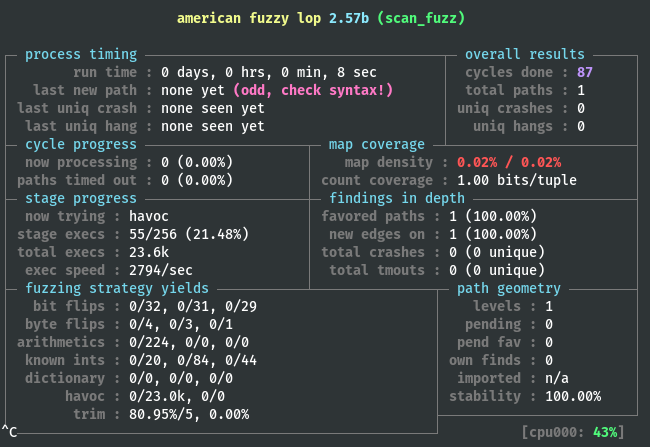
\includegraphics[width=0.8\textwidth]{afl-fuzz.png}}
\end{center}

Notice how last new path is highlighted, we could fix this with the steps proposed earlier.
When running on packages made to be fuzzed with AFL, I was able to get it working quite nicely
it is just the amount of preplanned thought and test-creation that must be done in order to 
use the tool effectively. 

\begin{center}
{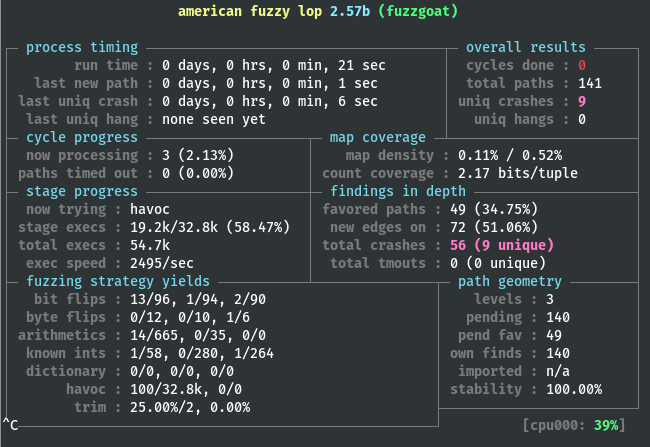
\includegraphics[width=0.8\textwidth]{afl-fuzz-pass.png}}
\end{center}

\section*{Final Notes}
The Mirai bot goes down in history as one of the most successful (in terms of users infected)
and carries its tasks out exactly as intended. As most pieces of malware, this one went on 
to spawn many strains, political chaos around the matter, and imposters taking credit. There
are many takeaways from analyzing this bug, the biggest being to use a secure password and 
enable SSH on capable devices. The bot operates on dictionary attacks so I think secure 
credentials are a huge step in preventing infection of not just this virus but many more. 
Based on the research and analysis of many sources, SSH was the common method of encryption that 
saw the least amound of attacks in comparison to insecure counterparts. 

\end{flushleft}
\end{sloppypar}
\end{document}
